This Section explains the method and principles used for the system integration process, between PyIceberg and \gls{HopsFS}. This Section is divided into three Subsections: Integration process, describing the activities to be conducted to integrate PyIceberg and \gls{HDFS}; Requirements; and Development environment, detailing the tools and resources that will be used during the integration process.


%%%%%  INTEGRATION PROCESS
\subsection{Integration process}
\label{subsec:integration_process}
The integration development process will follow an iterative in Figure \ref{fig:method_code_schema}. This project will require numerous interactions with \gls{HopsFS} maintainers (i.e., the industrial supervisors), since PyIceberg library has to interact with \gls{HopsFS}. This review process creates the need for a feedback loop, allowing the system to fit all the stakeholder requirements, described in Subsection~\ref{subsec:integration_reqs}. This process answers \gls{RQ}1, to which \glspl{G}1--2 are associated, as described in Section~\ref{sec:intro_goals}. The relationships between each process activity and \glspl{G} are here explained:

\begin{enumerate}
    \item \textbf{Set requirements collaboratively}: this activity is key for the completion of \glspl{G}1-2, as it is an initial system analysis, performed together with the industrial supervisors, who are knowledgeable on Hopsworks' infrastructure. This task sets the project requirements and investigates what needs to be integrated at a high-level abstraction.
    \item \textbf{Analyze system and tools}: this activity solves \gls{G}1 performing low-level code analysis on system and PyIceberg function calls, understanding what needs to be developed to integrate \gls{HopsFS} and PyIceberg. This activity is the first of an iterative loop accounting for the requirements fulfillment.
    \item \textbf{Develop integration}: this activity partially \gls{G}2, designing and developing a code solution from the information gathered during the analyses above.
    \item \textbf{Test integration}: this activity partially solves \gls{G}2, verifying the solution validity with integration tests. Failed integration tests or unfulfilled requirements will triggen a new loop iteration. Otherwise, the integretion process will be concluded.
\end{enumerate}

This process will produce a part of \gls{D}3, which is the code implementation for IcedHops, the PyIceberg and \gls{HopsFS} integration, including the consideration about the specific tools selected or discarded.

\begin{figure}[!t]
    \begin{center}
      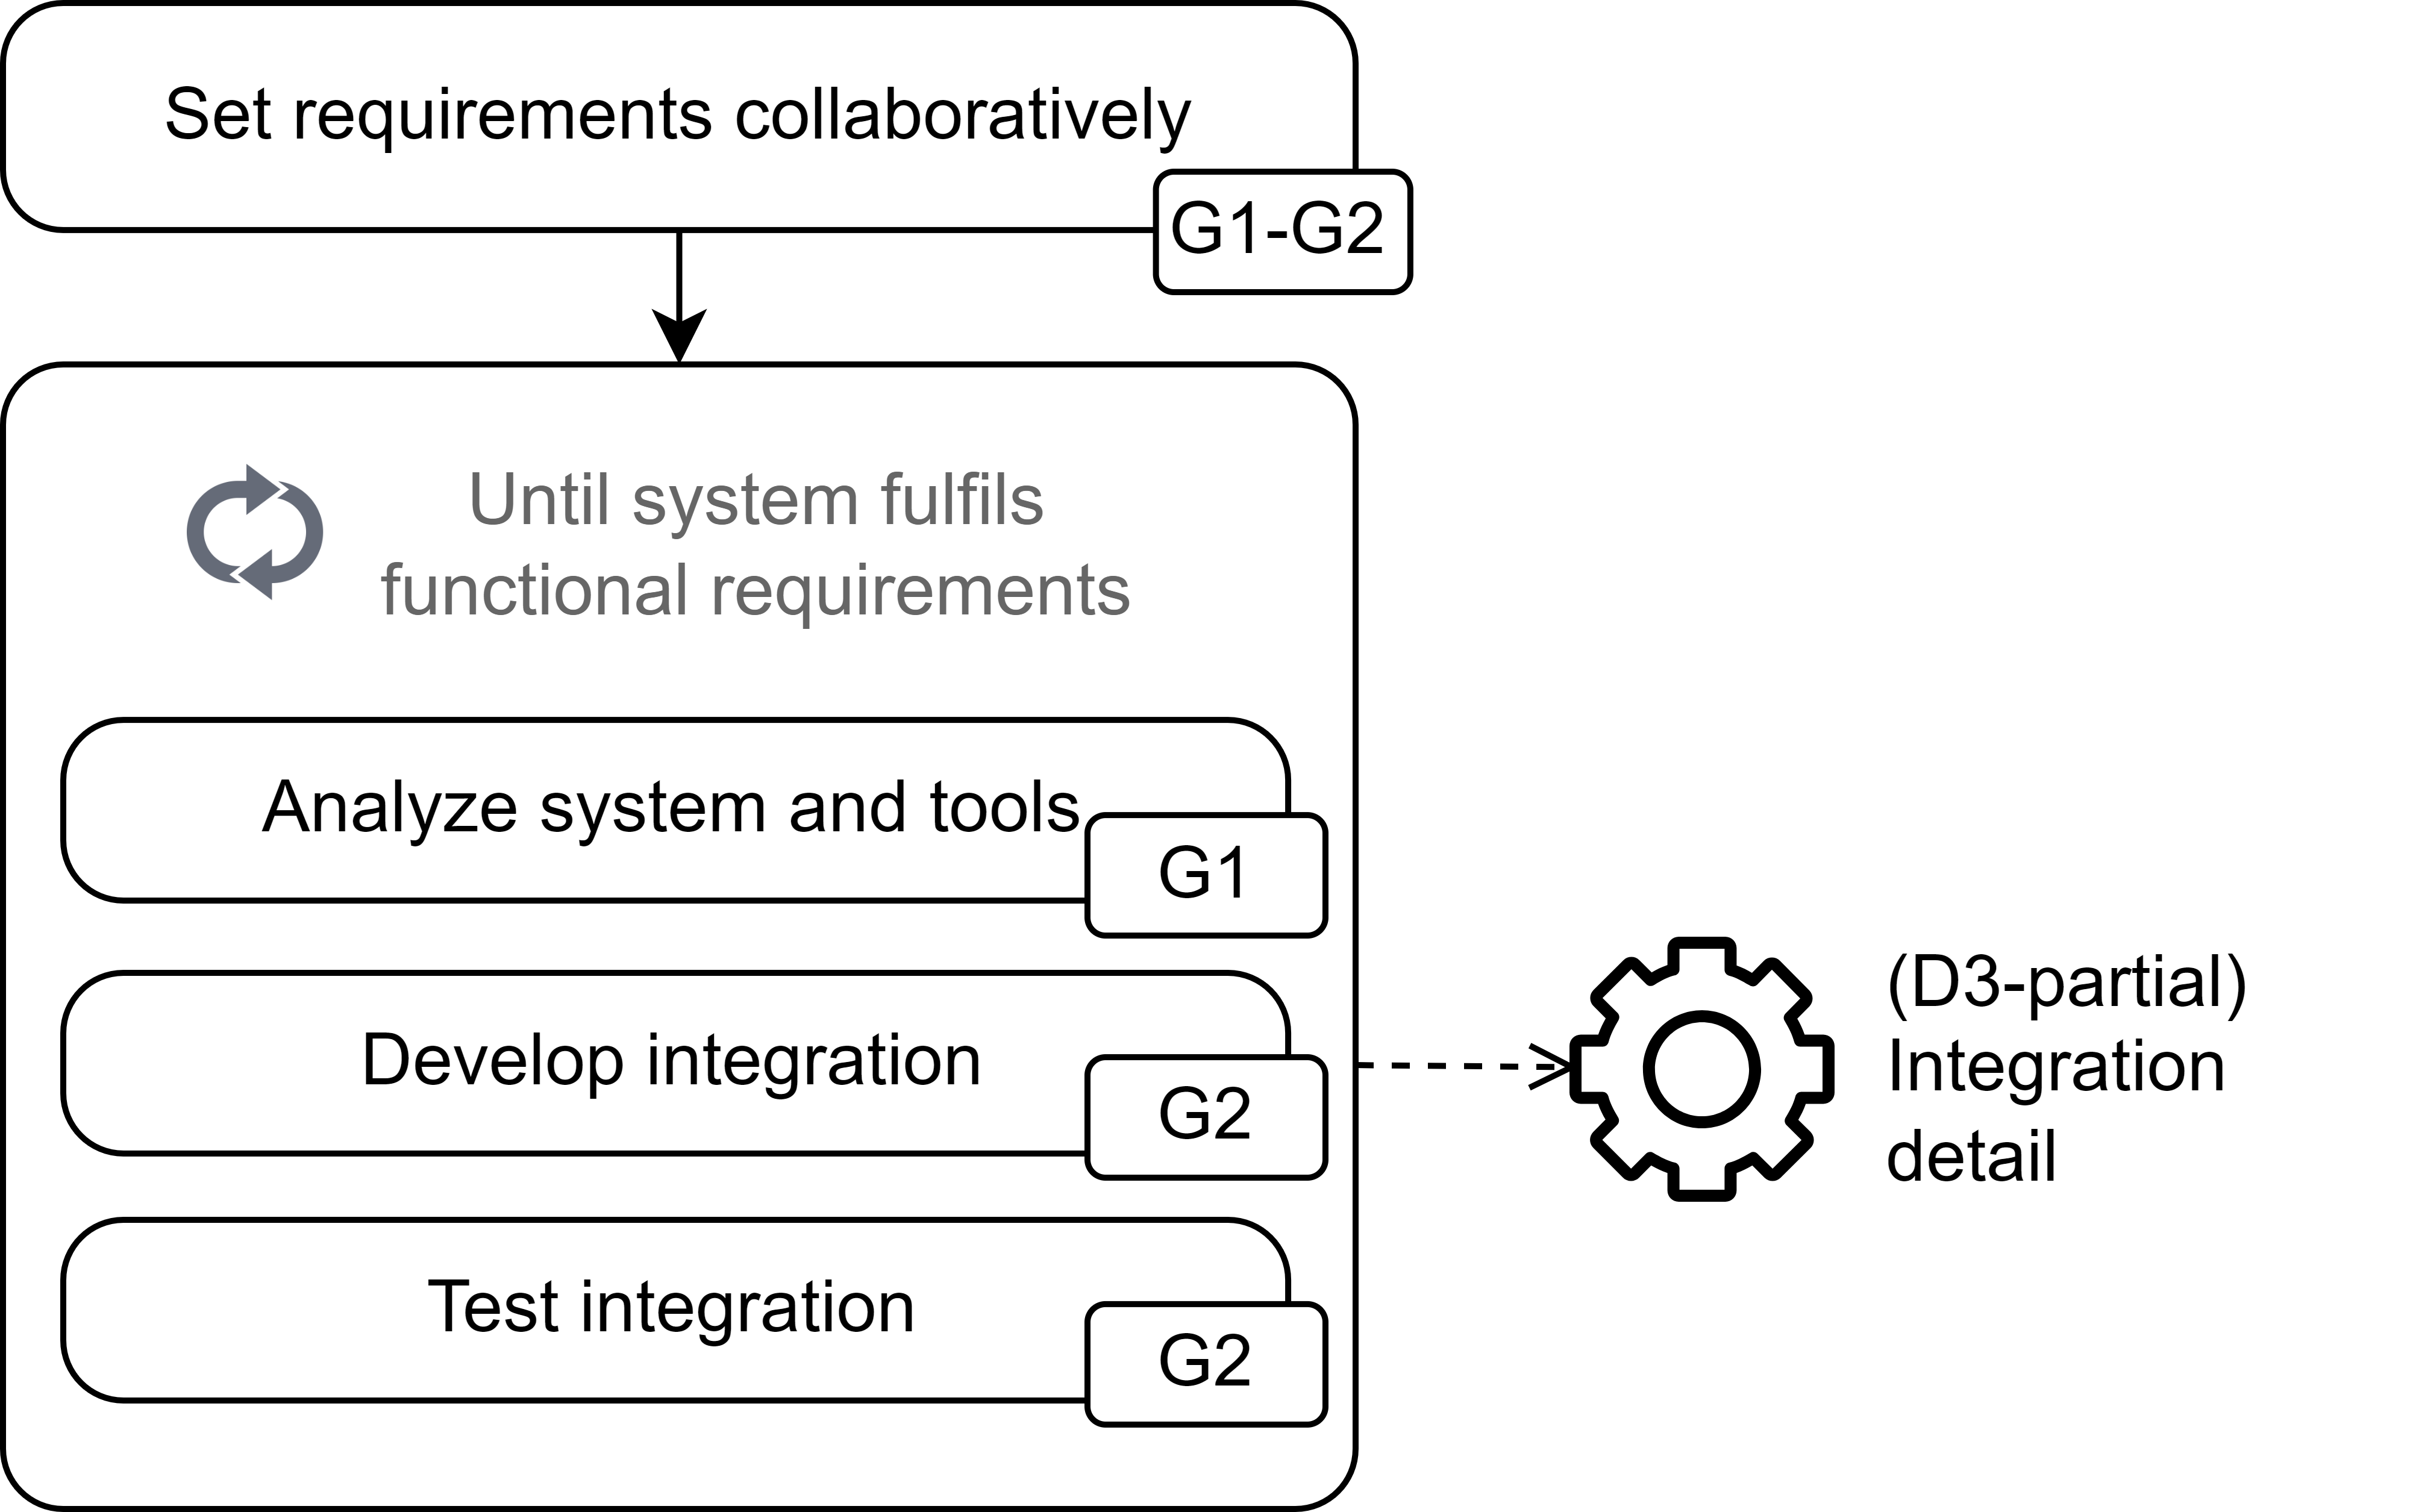
\includegraphics[width=0.8\textwidth]{figures/3-method/method_code.png}
    \caption[System integration process]{Diagram of the system integration process answering \gls{RQ}1. Each activity is associated to specific \glspl{G}. The process produces the integration detail (\gls{D}3 partial). The loop iterates until the functional requirements, defined in Section~\ref{subsec:integration_reqs}, are fulfilled.}
    \label{fig:method_code_schema}
    \end{center}
\end{figure}


%%%% REQUIREMENTS
\subsection{Requirements}
\label{subsec:integration_reqs}
A series of requirements are defined in agreement with Hopsworks AB, to create a solution that could be later used by the company, in a production environment. The \textbf{functional requirements} are:
\begin{enumerate}
    \item \textbf{Write Iceberg Tables}: the solution should allow to write Iceberg tables on \gls{HopsFS} via the PyIceberg library.
    \item \textbf{Read Iceberg Tables}: the solution should allow to read Iceberg tables on \gls{HopsFS} via the PyIceberg library.
\end{enumerate}
The \textbf{non-functional requirements} are:
\begin{enumerate}
    \item \textbf{Consistency}: the solution should be consistent with the current open-source codebase.
    \item \textbf{Maintainability}: the solution should minimize the need for maintenance and support.
    \item \textbf{Scalability}: the solution should handle read or write operations on Iceberg tables, up to 100 GB, to support small-scale dataset scenarios.
\end{enumerate}


%%%%% DEVELOPMENT ENVIRONMENT
\subsection{Development environment}
The system implementation will be developed using the following technologies:
\begin{itemize}
    \item \textbf{Computing resources}: the system integration will be developed on a \gls{VM} accessed via \gls{SSH} from a computer terminal. Local development will be avoided, due to low reproducibility and complexity of mounting \gls{HopsFS} on a local machine.
    \item \textbf{Code versioning and shared development}: GitHub will be used for versioning and sharing the developed solution.
\end{itemize}
